\pagestyle{fancy}
\fancyhead{} % clear all header fields
\fancyhead[LO,CE]{Conception logicielle}
\fancyhead[RO,LE]{2024-2025}
\chapter{Conception logicielle}

\section{Architecture logicielle}
L’application suit une architecture modulaire basée sur le MVVM(modèle-vue-vue modèle), divisée en trois couches principales :

\begin{itemize}
\item    Présentation (UI) : Gérée par des Composants Jetpack Compose et des ViewModels.

\item    Domain (Métier) : Contient les Use Cases et les interfaces de Repository.

\item    Data (Accès aux données) : Implémente les sources de données (Firebase, ESP32, Capteurs).
\end{itemize}

Pour des soucis de performance, les données envoyés aux microcontrôleurs sont des données de types booléennes, pour que l'éxecution se fait approximativement en temps réel. 


\section{Structure de la base de données dans Realtime Database}

L'application utilise une base de données de type \textit{clé-valeur} appelée \textbf{Realtime Database}, hébergée et gérée par Firebase. Cette base de données offre plusieurs avantages, tels qu'une infrastructure sans serveur, une haute disponibilité et une sécurité assurée par Google. La structure des données utilisée est illustrée à la figure~\ref{fig:structure_de_la_base_de_donnees}.

\begin{figure}[H]
   \centering
   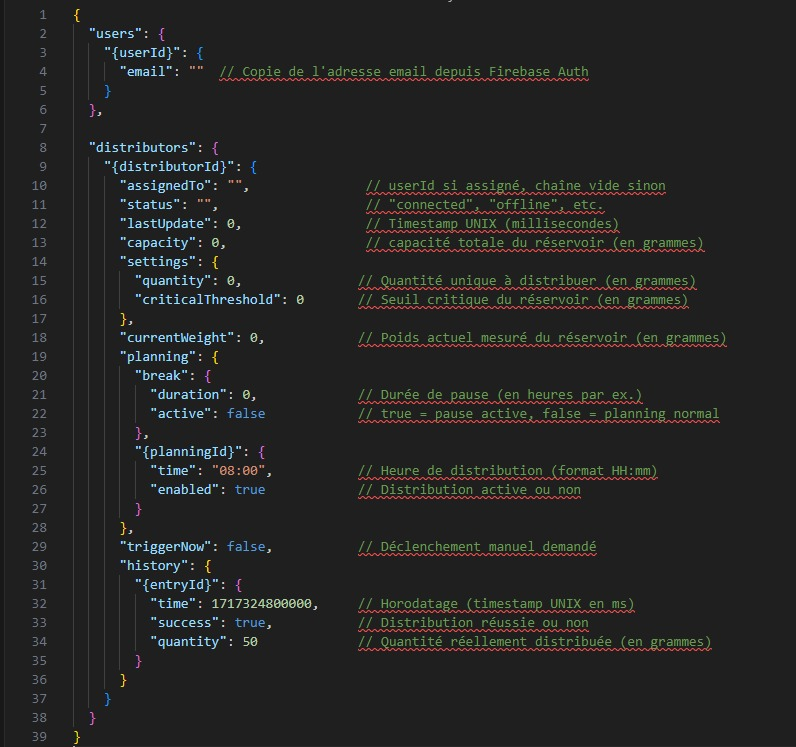
\includegraphics[scale=0.5]{dd3.jpeg}
   \caption{Structure de la base de données}
   \label{fig:structure_de_la_base_de_donnees}
\end{figure}

La base de données contient deux clés principales :

\begin{itemize}
\item \textbf{users} : contient les informations de tous les utilisateurs de l'application mobile.
\item \textbf{distributors} : contient les paramètres des distributeurs automatiques de nourriture pour chats.
\end{itemize}

\begin{enumerate}[label=\alph*)]
\item \textbf{Données des utilisateurs} 

\textbf{Firebase Authentication} est utilisé pour gérer l'authentification des utilisateurs. Les informations d'authentification sont stockées et gérées par ce service. Les données spécifiques à chaque utilisateur, stockées dans Realtime Database, sont :

\begin{itemize}
\item \textbf{\{userId\}} : identifiant unique généré par Firebase Authentication pour chaque utilisateur.
\item \textbf{email} : adresse e-mail utilisée par l'utilisateur pour se connecter à l'application.
\end{itemize}

\item{Données des distributeurs} 

Les données des distributeurs servent principalement à configurer leurs actions. Ces données incluent :

\begin{itemize}
\item \textbf{\{distributorId\}} : identifiant unique de chaque distributeur, généré lors de l'assemblage du matériel.
\item \textbf{assignedTo} : identifiant de l'utilisateur associé au distributeur.
\item \textbf{status} : état de la connexion Internet de l'ESP32.
\item \textbf{lastUpdate} : date de la dernière activité du distributeur.
\item \textbf{capacity} : capacité totale du réservoir en grammes.
\item \textbf{settings} : paramètres de distribution des croquettes, comprenant :
  \begin{itemize}
    \item \textit{quantity} : quantité à distribuer en grammes.
    \item \textit{criticalThreshold} : seuil critique du réservoir en grammes.
  \end{itemize}
\item \textbf{currentWeight} : poids actuel mesuré du réservoir en grammes.
\item \textbf{planning} : liste des distributions programmées par l'utilisateur. Chaque entrée contient :
  \begin{itemize}
    \item \textit{time} : heure de distribution au format \textit{HH:mm}.
    \item \textit{enabled} : indique si la distribution est active.
    \item \textit{break} : indique une pause dans la distribution.
  \end{itemize}
\item \textbf{triggerNow} : booléen indiquant un déclenchement manuel du distributeur.
\item \textbf{history} : historique des distributions effectuées.
\end{itemize}



\end{enumerate}

\section{Composants clés de l’application} 

\subsection{Gestion des utilisateurs (Firebase Auth)}
L'inscription et la connexion se fait via email et mot de passe. Seul l’utilisateur authentifié peut contrôler son distributeur.

\subsection{Programmation des repas} 
Les horaires de distributions et la quantité sont stockés dans Firebase avec \textbf{Real Time Database}.

\subsection{Contrôle manuel}
On envoi une commande depuis Firebase qui provoque un déclenchement immédiat sur l’ESP32. Un "trigger" de type booléen qui permet au microcontrôleur d'effectuer  ou non une action sur l'ensemble du système.

\subsection{Notifications}
Des alertes sont envoyés, comme la confirmation de la nourriture distribuée et le niveau de nourriture faible. Ces notifications viennent de l'application mobile, qui envoi un "trigger"


\pagestyle{fancy}
\fancyhead{} % clear all header fields
\fancyhead[LO,CE]{Conception électronique}
\fancyhead[RO,LE]{2024-2025}
\chapter{Conception électronique}
\section{Présentation matériel}
Ce projet a comme partie électronique les composants suivant : pour le microcontrôleur nous avons utilisés l'ESP32, 2 capteurs de poids avec muni convertisseur analogique vers numérique de 24 bits le HX711, et d'un servomoteur.

\begin{itemize}
\item \underline{\textbf{le microcontrôleur}:} L’ESP32 est un microcontrôleur à faible consommation d’énergie, doté d’un processeur double cœur 32 bits, de connexions Wi-Fi et Bluetooth intégrées. Il est largement utilisé pour les projets IoT (Internet des Objets) grâce à sa puissance de calcul, sa connectivité sans fil, ses nombreux broches. Pour ce projet, le dispositif est doté de l'ESP32 WROOM-32 DevKit à 38 broches.\\


\begin{figure}[H]
	\centering
	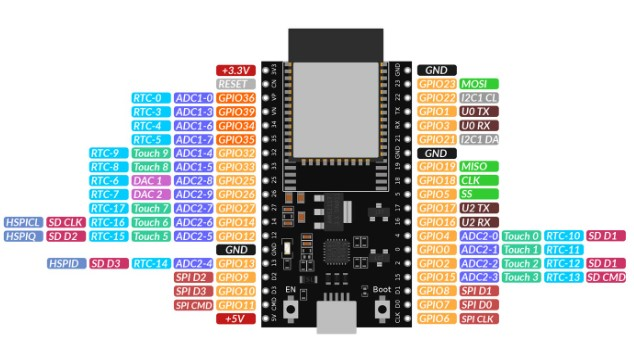
\includegraphics[scale=0.8]{1.jpg}
	\caption{Brochage de l'ESP32 WROOM-32 DevKit}
\end{figure}

\item \underline{\textbf{les capteurs de poids}:} Ils utilisent des jauges de contrainte montées sur une cellule de charge pour détecter les déformations causées par une masse. Le HX711 est un convertisseur analogique-numérique (ADC) va amplifier et lire les signaux analogique de faible amplitude que va généré la cellule de charge. Ici, le dispositif utilise 2 capteurs de masse différentes l'un de 1kg et l'autre de 20kg pour le réservoir.

\begin{figure}[H]
	\centering
	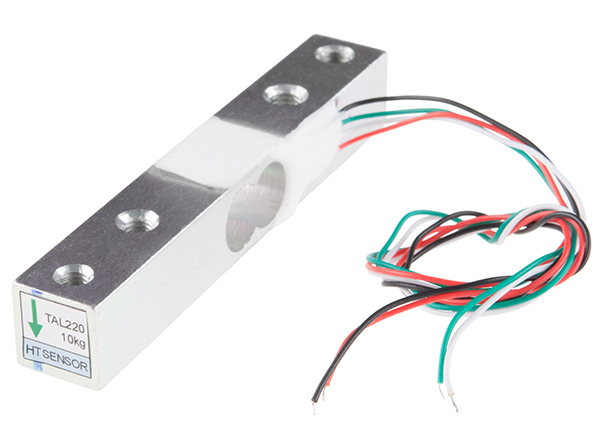
\includegraphics[scale=0.8]{2.jpg}
	\caption{Cellule de charge}
\end{figure}

\begin{figure}[H]
	\centering
	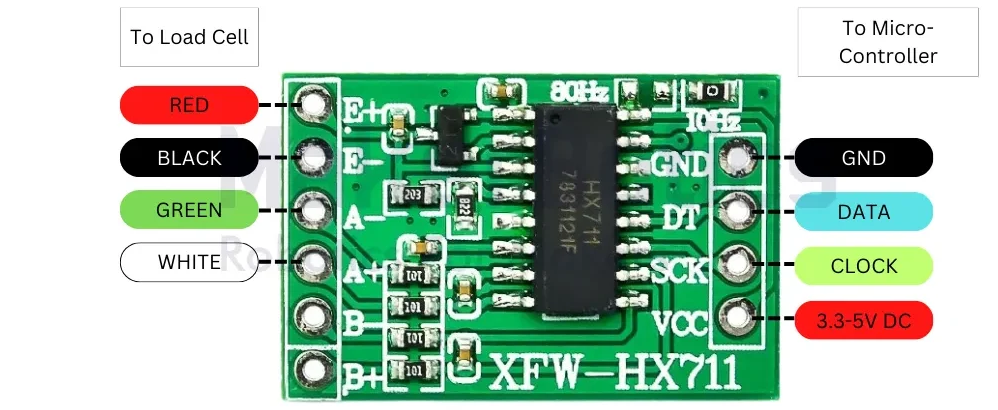
\includegraphics[scale=0.5]{1.png}
	\caption{Brochage du HX711}
\end{figure}

\item \underline{\textbf{le servo-moteur}:} C'est un moteur contrôlé en position, utilisé pour effectuer des rotations précises dans une plage définie (souvent 0° à 180°). Il reçoit un signal PWM (modulation de largeur d’impulsion), la largeur de l’impulsion détermine ainsi l’angle de rotation. Le servo-moteur servira d'ouverture de vanne dans notre cas.

\begin{figure}[H]
	\centering
	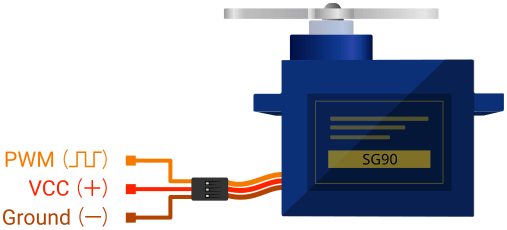
\includegraphics[scale=0.5]{2.png}
	\caption{Brochage du servo-moteur}
\end{figure}

\item  \underline{\textbf{Communication entre le microcontrôleur et le websocket}:} Pour récuperer les données depuis Firebase et le transmettre à l'ESP32, nous avons mis en place un serveur websocket, qui permet entre outre de recevoir des messages contenant des données depuis l'ESP32.  Le serveur websocket va ensuite les tranférer les données  vers  Real Time Database de Firebase.

\begin{figure}[H]
	\centering
	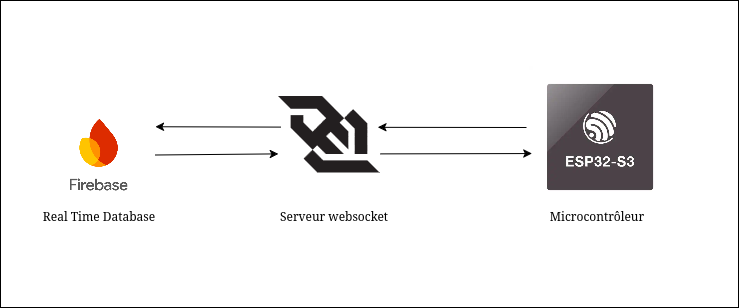
\includegraphics[scale=0.5]{4.png}
	\caption{Communication entre Firebase, le serveur websocket et l'ESP32}
\end{figure}

\end{itemize}


\section{Schéma d'ensemble du circuit}
Malheureusement, pas de beaucoup de logiciels peuvent simuler l'ESP32 et montrer précisement le schéma électronique du projet. Néanmoins, la platforme \textit{Wokwi}, permet cela, c'est une plateforme web qui permet de simuler à quelques détails près L'ESP32, et il nous fournit un schéma d'ensemble avec.\\[0.3cm]

\begin{figure}[H]
	\centering
	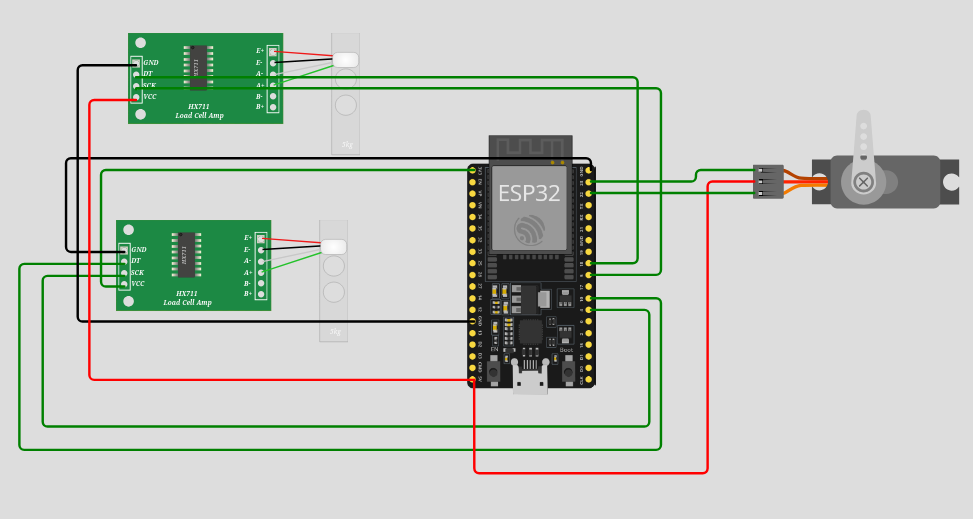
\includegraphics[scale=0.5]{3.png}
	\caption{Schéma d'ensemble du dispositif}
\end{figure}


\pagestyle{fancy}
\fancyhead{} % clear all header fields
\fancyhead[LO,CE]{Réalisation}
\fancyhead[RO,LE]{2024-2025}
\chapter{Réalisation}













\pagestyle{fancy}
\fancyhead{} % clear all header fields
\fancyhead[LO,CE]{Tests et validation}
\fancyhead[RO,LE]{2024-2025}
\chapter{Tests et validation}
